%% AULA 1
%\section{Aula 1}

\begin{frame}{O que é o \TeX?}
\begin{itemize}
\item \prog{\TeX} é um programa criado por Donald E.~Knuth, usado para desenvolvimento de documentos;
\item Formatador de documentos (como troff e groff -- programas hoje obsoletos);
\end{itemize}
\end{frame}

\begin{frame}{O que faz o \TeX?}
\begin{itemize}
\item Permite desenvolver documentos complexos, incluindo facilidades
  para:
  \begin{itemize}
\item Gerar sumário, index, lista de figuras, lista de 
  tabelas e referências bibliográficas;
\item Importar e tratar imagens de vários formatos  (escalando, rotacionando, convertendo, etc.);
\item Desenvolver gráficos diagramáticos;
\item Representar partituras musicais, partidas de xadrez, fórmulas químicas etc.
\end{itemize}
\end{itemize}

\begin{block}{O poder do \TeX}
O poder do \TeX\ reside em sua habilidade de tratar textos técnicos complicados e exibir fórmulas matemáticas.
\end{block}
\end{frame}

\begin{frame}{Vantagens}
\begin{itemize}
\item Qualidade tipográfica superior (fontes e distribuição do texto
  na página);
\item Compatibilidade (Donald Knuth ``congelou'' o
  programa \TeX);
\item Estabilidade e ausência de falhas (uso prolongado \newline do mesmo programa virtualmente
  eliminou todos os erros);
\item Padrão adotado pela \emph{American Mathematical \newline Society} para
  comunicação entre matemáticos.
\end{itemize}
\end{frame}

\begin{frame}{Formatos usados por \TeX}
\begin{itemize}
\item Os formatos usados por \TeX\ permitem sua livre distribuição (formatos abertos -- TEX, DVI e PDF);
\item Converte para outros formatos (PS, HTML e XML);
\item Existe completa compatibilidade dos documentos.
\end{itemize}
\end{frame}

\begin{frame}{Outras características de \TeX}
\begin{itemize}
\item \TeX\ é multiplataforma (existe para virtualmente qualquer máquina e sistema operacional);
\item \TeX\ enfatiza o \emph{projeto lógico de documentos};
\item \TeX\ é modular;
\item Os recursos do \TeX{} podem ser extendidos pela adição de macros.
\end{itemize}
\end{frame}


\begin{frame}{O que é \LaTeX?}
\begin{itemize}
\item \LaTeX\ é um conjunto padrão de macros para \TeX\ que permite
  um aumento da produtividade no uso do programa;
\item Mais macros podem ser incluidas por meio de pacotes (por exemplo: \Xy-pic, MusiX\TeX, CircuiTikz, etc.);
\item Programas externos, desenvolvidos por programadores e usuários
  de \TeX, extenderam as funcionalidades (por exemplo: BiB\TeX,
  makeindex, etc.).
\end{itemize}
\end{frame}

\begin{frame}{Abordagens para o projeto de documentos}
\begin{itemize}
\item Projeto visual $\times$ projeto lógico de documentos:
\begin{itemize}
\item Projeto visual enfatiza o estético e envolve grande esforço de formatação;
\item Projeto lógico enfatiza a estrutura e economiza tempo pois a formatação é consequência da estrutura;
\item Projeto lógico provoca uma reflexão sobre o texto que tem consequências benéficas até sobre o conteúdo sendo desenvolvido;
\end{itemize}
\end{itemize}
\end{frame}

\begin{frame}{Comparação entre processador de textos e \TeX}
Fórmula obtida usando-se um processador de textos típico:
\begin{center}
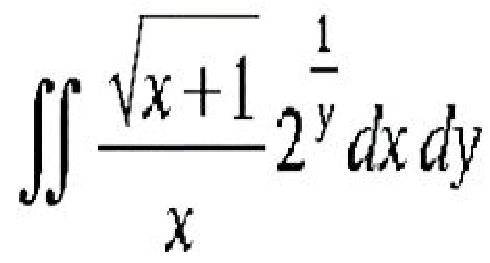
\includegraphics[width=0.5\textwidth]{img/integral.pdf}
\end{center}

Fórmula obtida usando-se \TeX:
\[\int\!\!\!\int\frac{\sqrt{x+1}}{x}2^{\frac{1}{y}}\mathrm{d}x\,\mathrm{d}y\]
\end{frame}

\begin{frame}{Projeto visual $\times$ lógico}
\begin{description}
	\item [Projeto visual] baseado em menus e botões  (o usuário ``desenha'' a fórmula/texto);
	\item [Projeto lógico] baseado em comandos:
\end{description}
	
	\begin{LaTeXcode}[Comandos]
	\string\[\LCmd{int}\string\!\string\!\string\!\LCmd{int}
	\LCmdArg{frac}{\LCmdArg{sqrt}{x+1}}\Larg{x}2\string^\{
	 \LCmdArg{frac}{1}\Larg{y}\}\n
	 \LCmdArg{mathrm}{d}x\string\,\LCmdArg{mathrm}{d}y\string\]
	\end{LaTeXcode}

Produz:
	\begin{LaTeXoutput}[]
	\[\int\!\!\!\int\frac{\sqrt{x+1}}{x}2^{\frac{1}{y}}\mathrm{d}x\,\mathrm{d}y\]
    \end{LaTeXoutput}
\end{frame}

\begin{frame}{Observações}
\begin{itemize}
\item \texttt{\string\[ } e \texttt{\string\]} -- entra e sai do modo matemático;
\item \LCmd{int} -- integral;
\item \texttt{\string\!} -- espaço negativo (para obter o espaçamento correto na integral dupla) -- poderia ter sido usado o comando \LCmd{iint};
\item \LCmdArg{frac}{\ldots}\Larg{\ldots} -- fração;
\item \LCmdArg{sqrt}{\ldots} -- raiz quadrada;
\item \texttt{\string^} -- expoente;
\item \texttt{\string\,} -- espaço pequeno;
\item \LCmdArg{mathrm}{\ldots} -- fonte romano do modo matemático.
\end{itemize}
\end{frame}

\begin{frame}{Projeto lógico}
\begin{itemize}
	\item No projecto lógico, o aspecto estético depende do contexto/estrutura (por 
	exemplo, se a fórmula está dentro de um parágrafo ou destacada do parágrafo). 
	Exemplo:
	\begin{itemize}
		\item O somatório $\sum_{i=0}^\infty a_i/2$ resulta em \dots		
		\item O somatório \[\sum_{i=0}^\infty \frac{a_i}{2}\] resulta em \dots
	\end{itemize}
\end{itemize}
\end{frame}

\begin{frame}{Autor, designer e tipógrafo}
\begin{itemize}
\item Tipografia tradicional: autor $\longrightarrow$ designer $\longrightarrow$ tipógrafo;
\item Designer: responsável pelo layout do documento (escolha dos fontes, número de colunas, margens, etc.). Trabalha baseado em sua percepção do que o autor deseja e em seu conhecimento das regras da tipografia (que privilegiam a facilidade de leitura e não a beleza estética);
\item Tipógrafo: interpreta as anotações geradas pelo designer e produz a matriz para impressão do documento.
\end{itemize}
\end{frame}

\begin{frame}{Tipografia}
\centering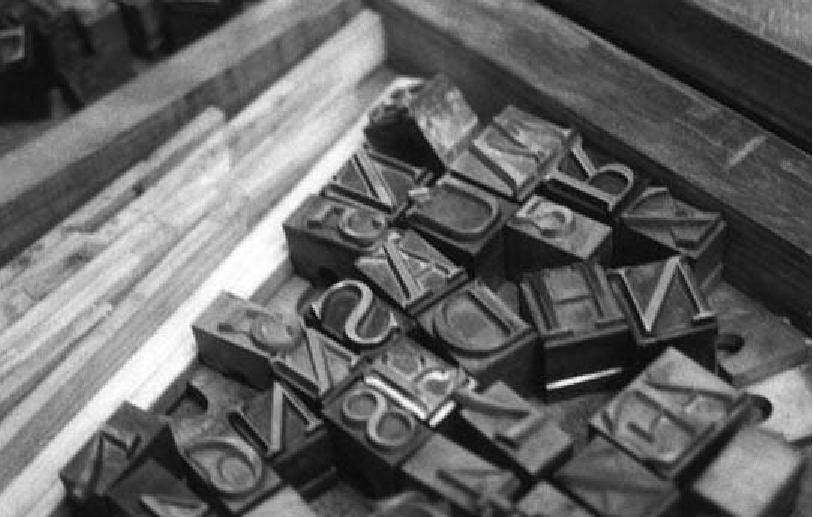
\includegraphics[width=0.85\textwidth]{img/tipografia.pdf}
\end{frame}

\begin{frame}{Funcionamento do \TeX{} e \LaTeX}
\begin{itemize}
\item \LaTeX\ interpreta o papel do designer;
\item \TeX\ interpreta o papel do tipógrafo.
\end{itemize}
\end{frame}

\begin{frame}{\TeX\ e \texttt{pdftex} como um compilador}
\begin{itemize}
\item O programa \TeX\ é um compilador que lê um arquivo de entrada (.TEX) e produz um arquivo de saída (.DVI ou .PDF);
\item O arquivo .TEX é um arquivo ASCII que contém o texto acrescido de comandos ou macros \TeX\ e \LaTeX;
\item O arquivo .DVI usa um formato independente de dispositivo e que pode ser impresso, visualizado ou convertido para outros formatos;
\item Nas versões modernas de \TeX\ o programa de compilação é o \texttt{pdftex}, que pode produzir tanto um arquivo .DVI quanto um arquivo .PDF (Portable Document Format), o qual apresenta vantagens se comparado com o formato DVI -- tornando o formato DVI um pouco obsoleto.
\end{itemize}
\end{frame}

\begin{frame}{Os comandos do \LaTeX}
\begin{itemize}
	\item Os comandos são necessários para que \LaTeX\ possa formatar o texto 
	(\LaTeX\ não é tão inteligente como um designer/tipógrafo humano);
	%
	\item Os comandos \TeX\ normalmente são antecedidos de 
	``\texttt{\textbackslash}'' (por exemplo, para obter \LaTeX\ deve-se digitar 
	\LCmd{LaTeX} e para obter ``\textbackslash'' 	deve-se digitar 
	\texttt{\$}\LCmd{backslash}\texttt{\$} ou \LCmd{textbackslash});
	%
	\item A linguagem \TeX\ segue as regras/ideias de linguagens de programação 
	(declarações e corpo do programa; ligação de bibliotecas; regras de escopo; 
	etc.);
\end{itemize}
	
    \begin{block}{Observação}
    Maiúsculas $\neq$ minúsculas.
    \end{block}
\end{frame}

\begin{frame}{Como funciona o processo de compilação}
\begin{itemize}
\item  \LaTeX{} funciona como um compilador de uma passagem, gerando ao final do processo de compilação um arquivo .AUX que será lido no início da próxima execução do programa;
\item Por isto, frequentemente é necessário compilar mais de uma vez o fonte para resolver todas as pendências;
\item Ao final da execução de \LaTeX, é gerado também um arquivo .LOG contendo informações sobre a compilação.
\end{itemize}
\end{frame}

\begin{frame}{Editando o documento \TeX}
Existem diversos editores ASCII que se adaptam bem para o uso com \TeX: \prog{Emacs}, \prog{TeXmaker}, \prog{\TeX{works}}, \prog{TeXstudio}, \prog{TeXShop}, \prog{WinEdt}, \prog{\TeX{}nicCenter}, etc.
\end{frame}

\begin{frame}{Emacs}
\begin{itemize}
\item Editor disponível para Linux, Windows e MacOS, entre outras plataformas;
\item Veja: \url{http://www.gnu.org/software/emacs/}

\vspace{0.3cm}

\centering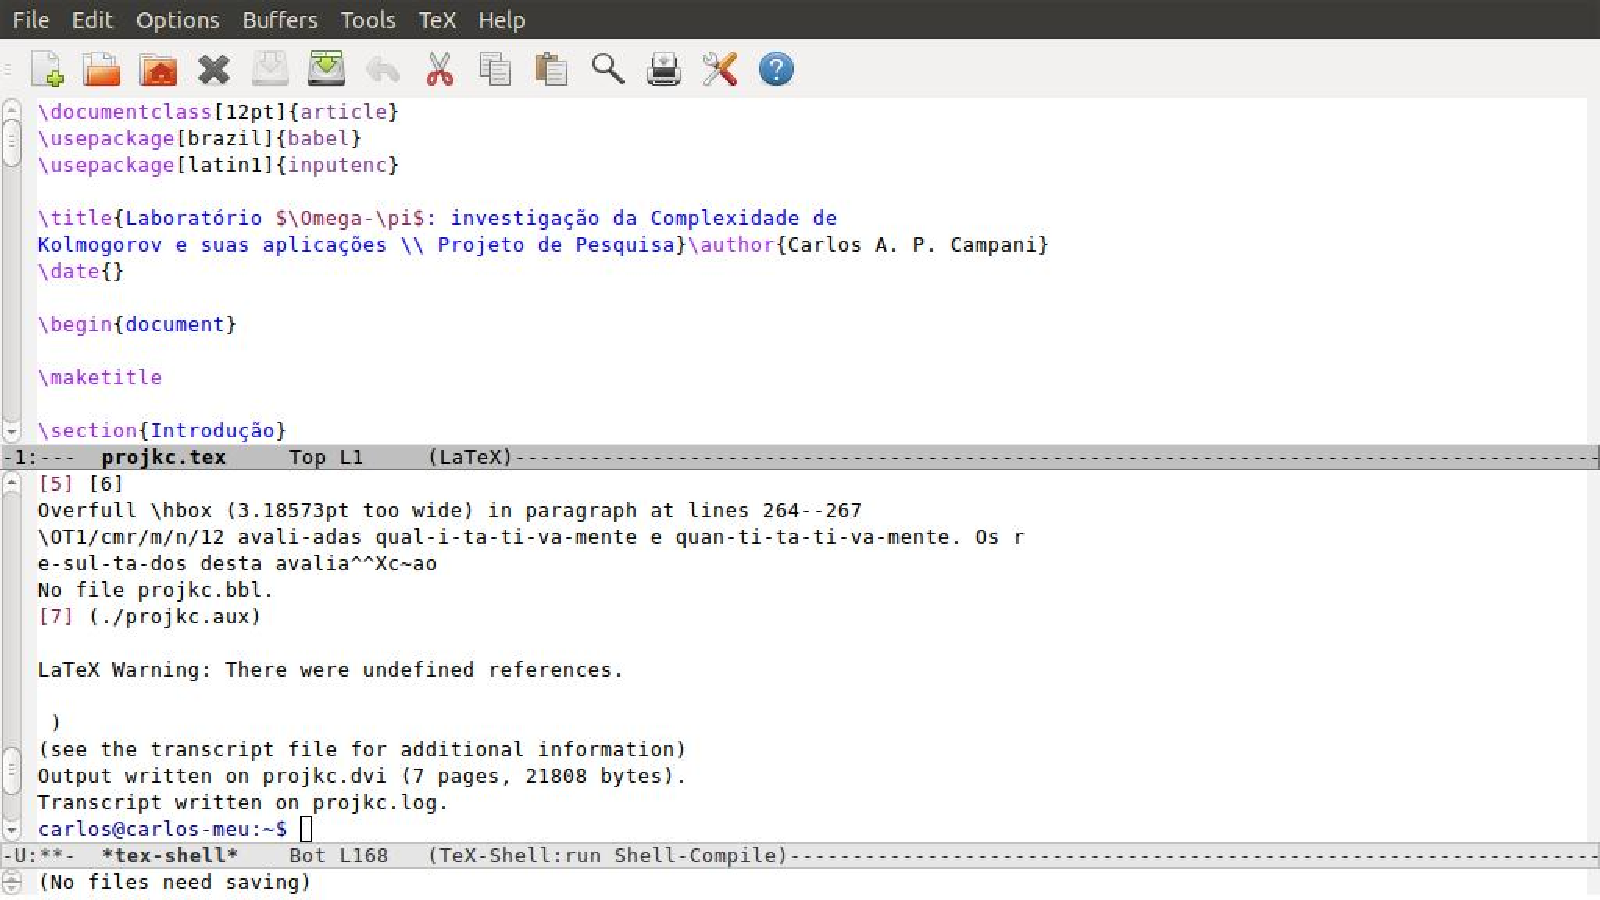
\includegraphics[width=0.85\textwidth]{img/emacs.pdf}
\end{itemize}
\end{frame}

\begin{frame}{TeXmaker}
\begin{itemize}
\item Disponível para Linux, Windows e MacOS
\item Veja: \url{http://www.xm1math.net/texmaker/}

\vspace{0.5cm}

\centering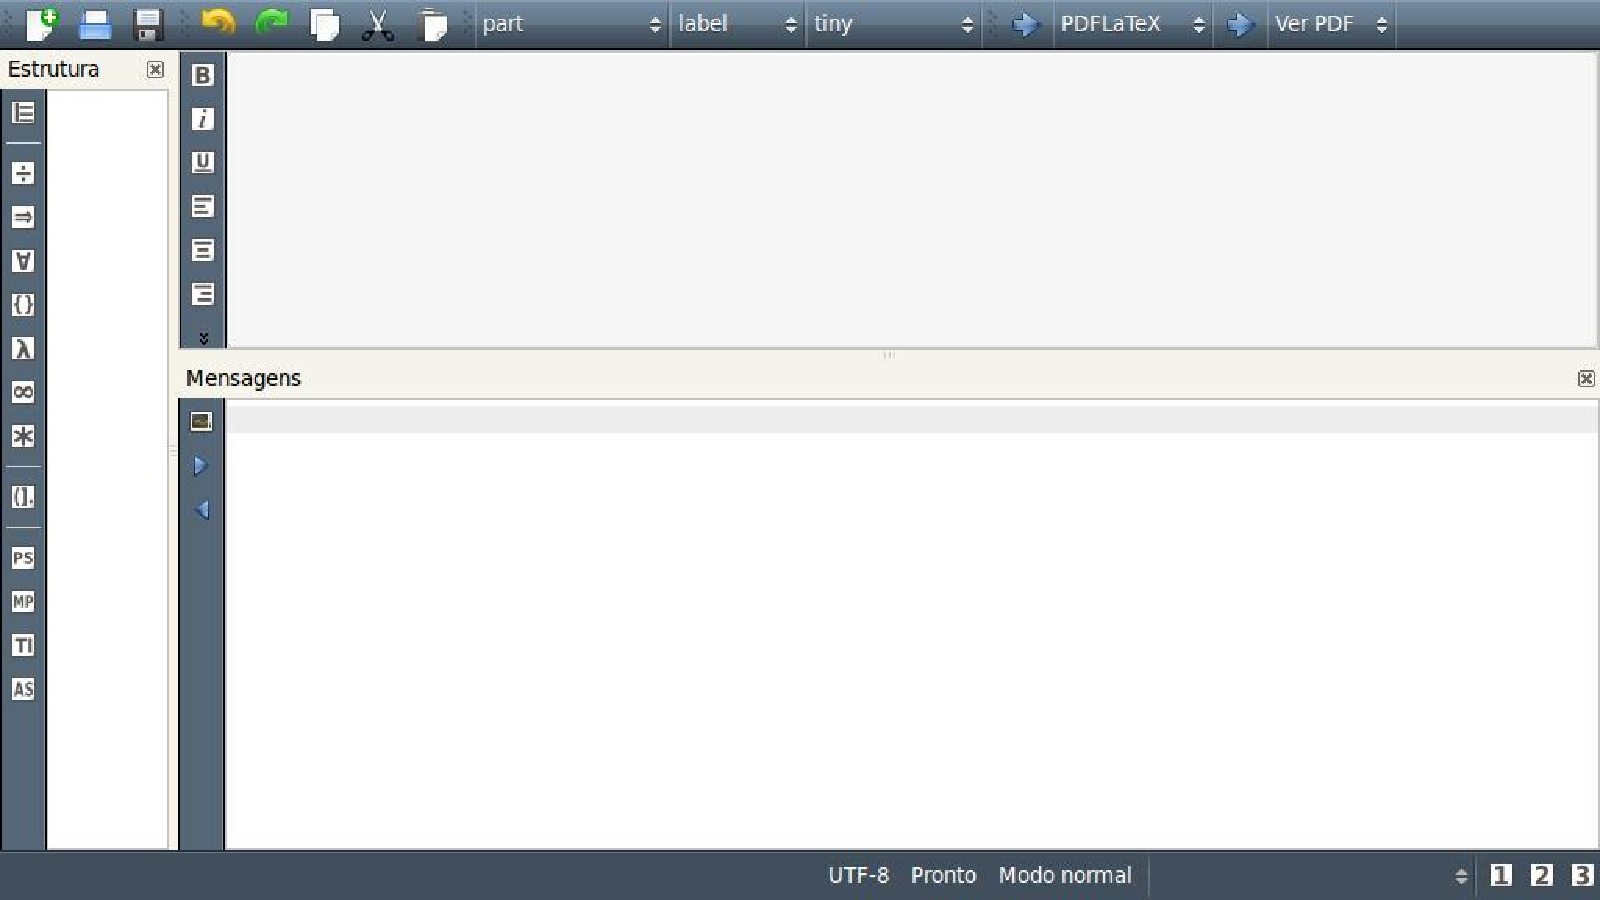
\includegraphics[width=0.85\textwidth]{img/texmaker.pdf}
\end{itemize}
\end{frame}

\begin{frame}{\TeX{works}}
\begin{itemize}
\item Disponível para Linux, Windows e MacOS
\item Veja: \url{http://www.tug.org/texworks/}

\vspace{0.25cm}

\centering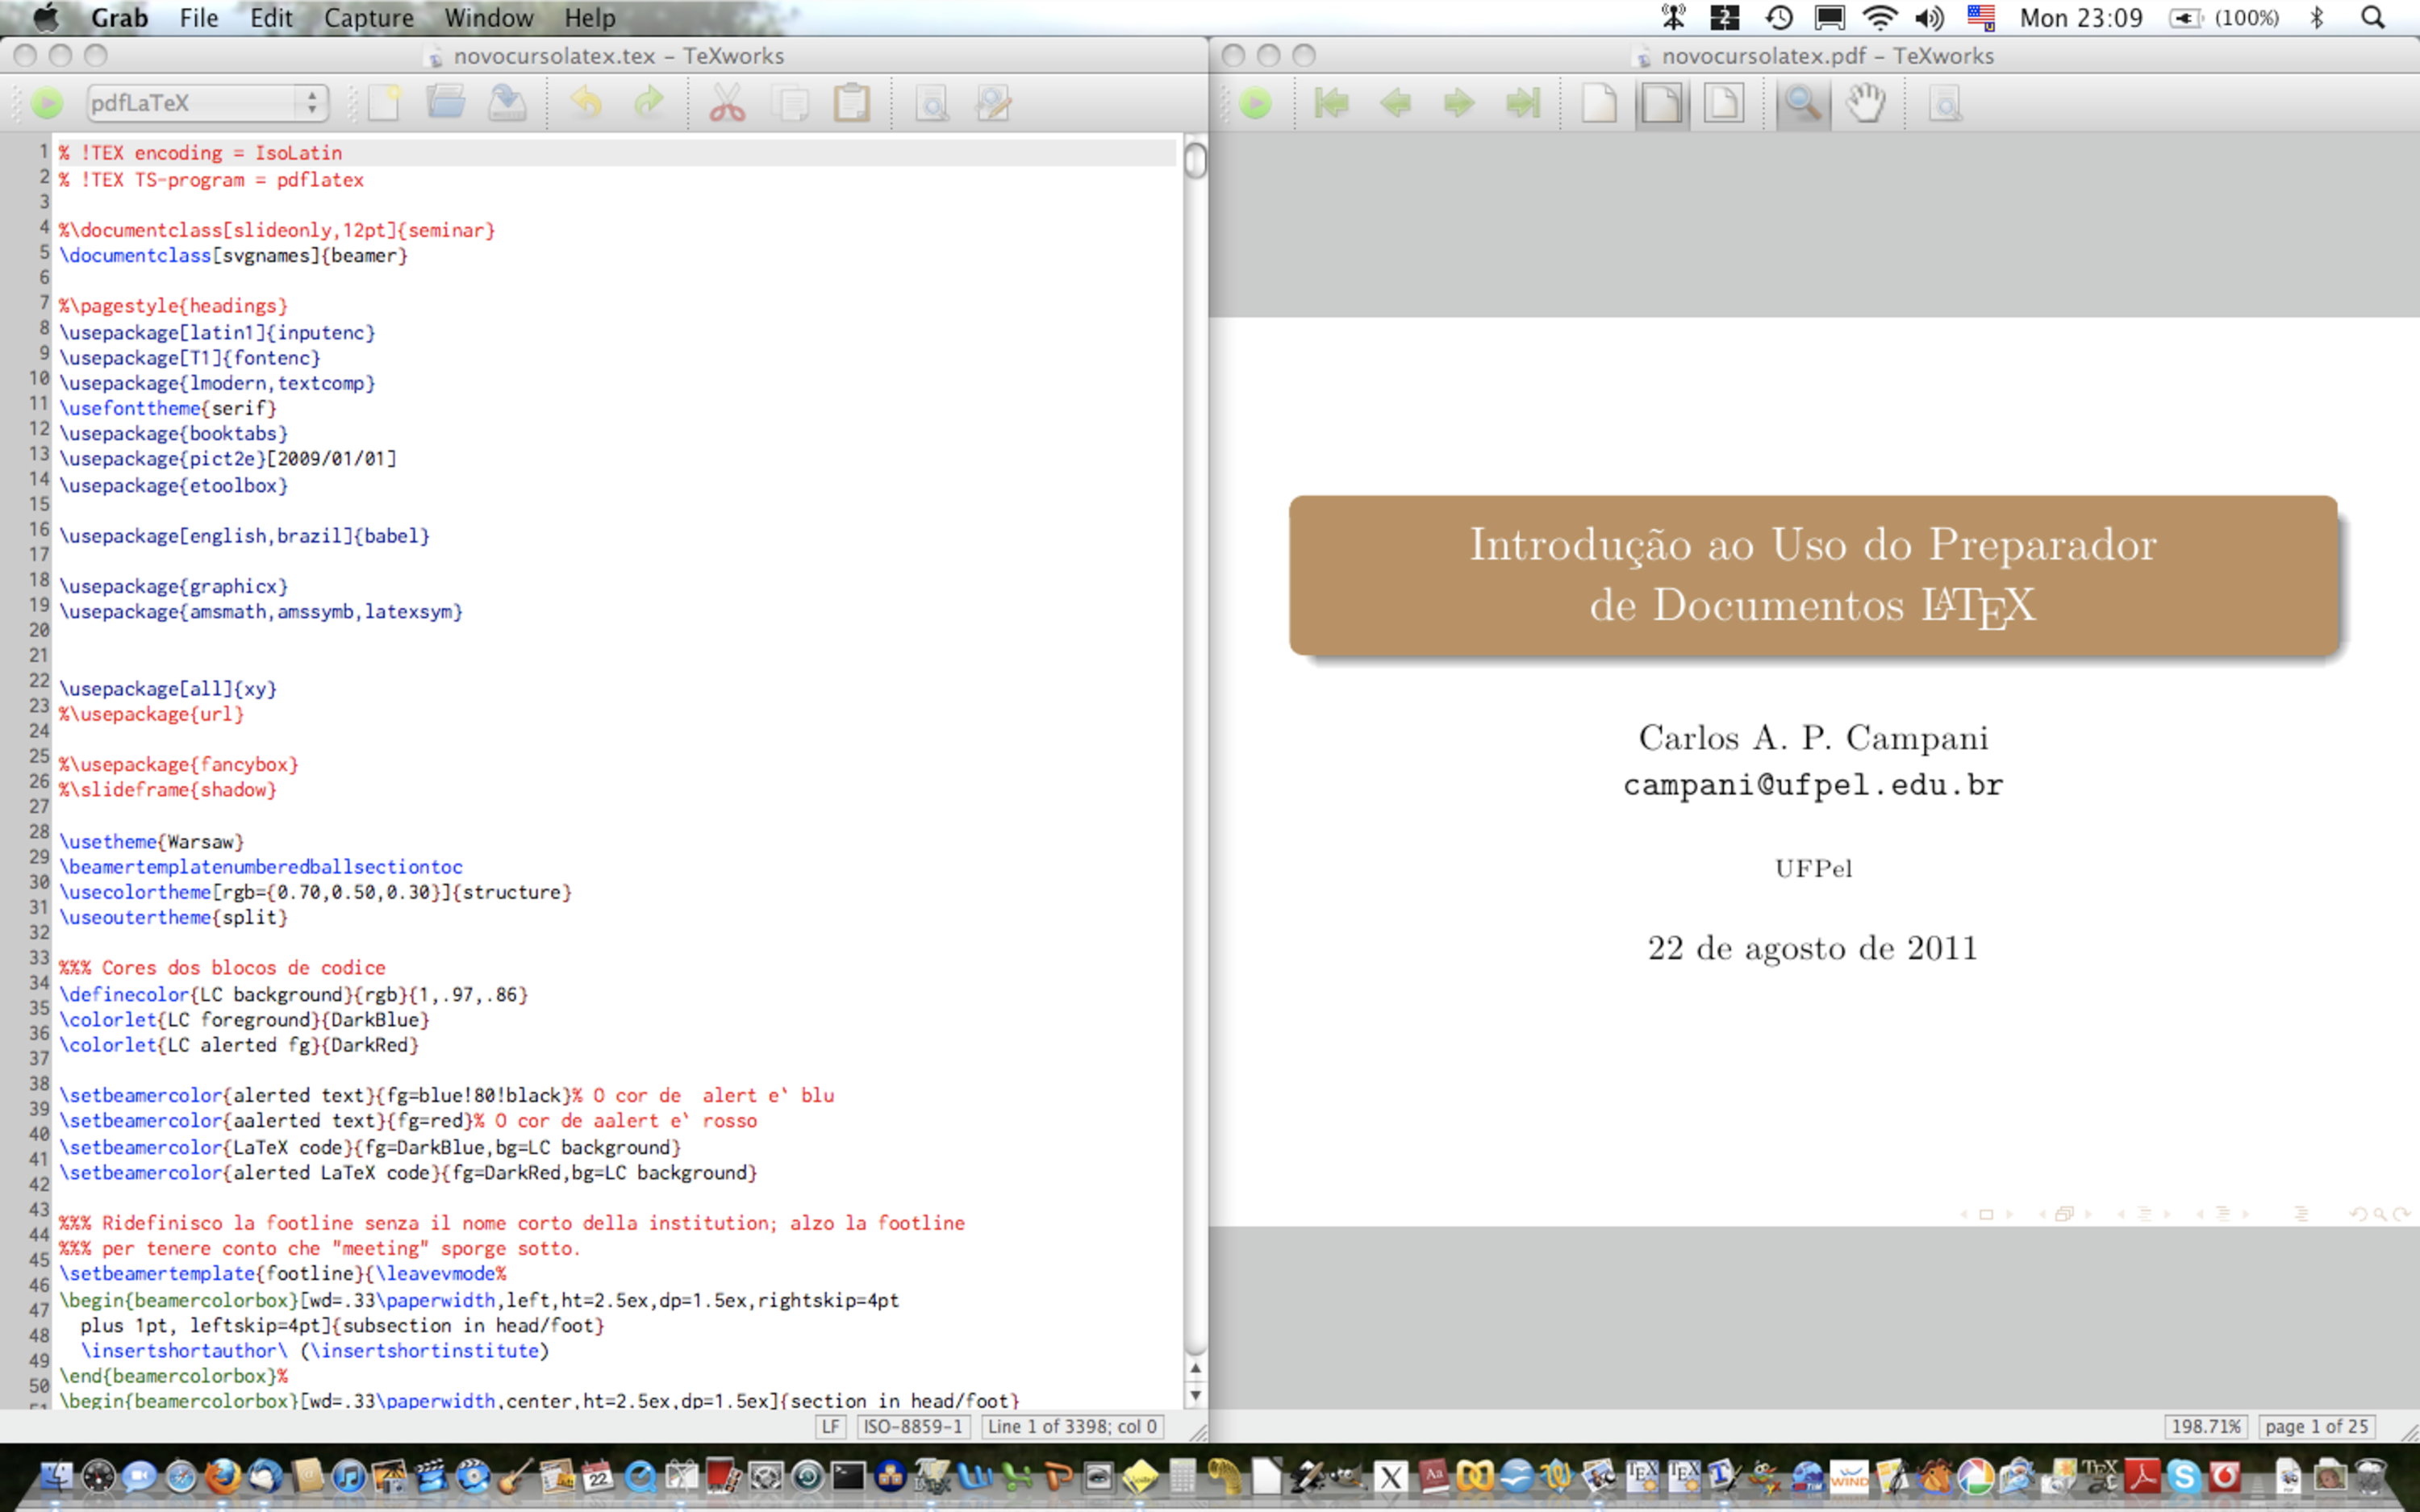
\includegraphics[width=0.80\textwidth]{img/TeXworksPDF.pdf}
\end{itemize}
\end{frame}


\begin{frame}{TeXShop}
\begin{itemize}
\item Disponível somente para MacOS
\item Instalado com Mac\TeX.
\end{itemize}

\centering
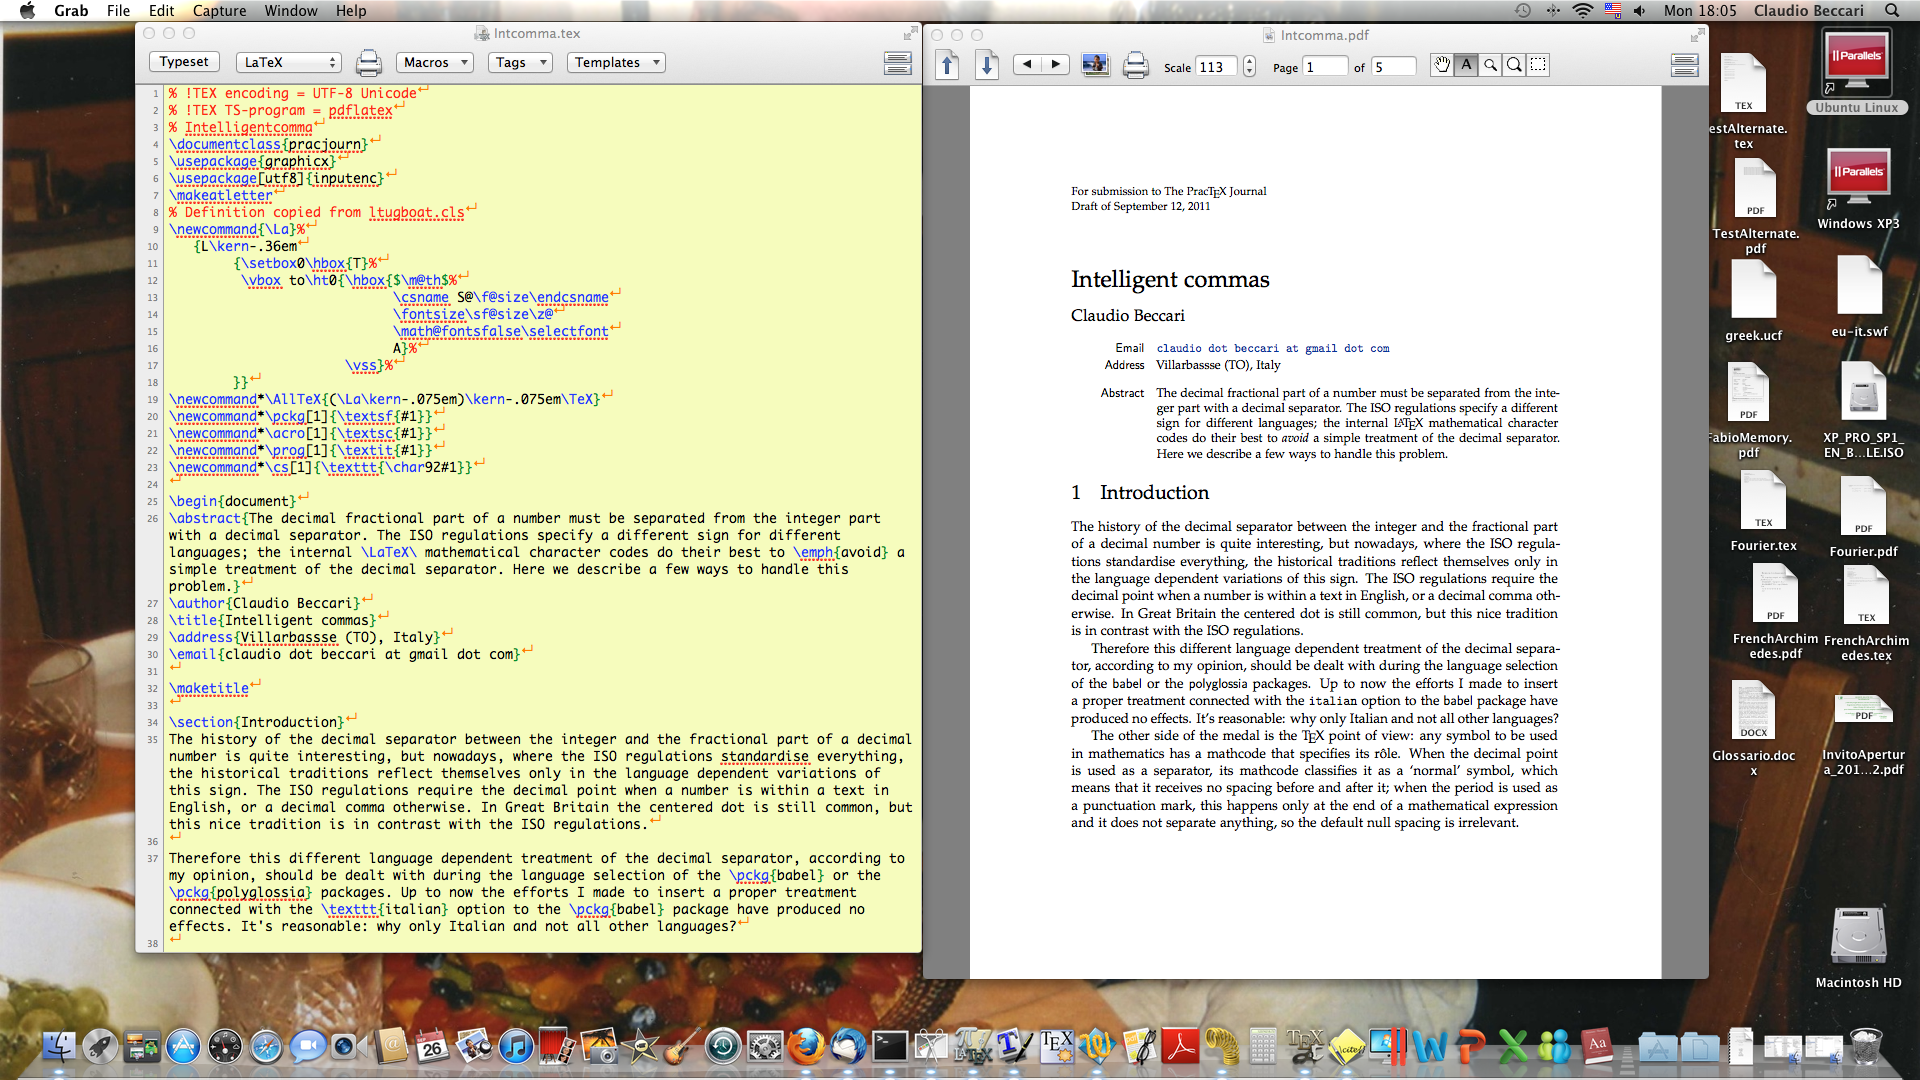
\includegraphics[width=\textwidth,height=.7\textheight,keepaspectratio]{img/TeXShopPNG.png}
\end{frame}

\begin{frame}{WinEdt}
\begin{itemize}
\item Programa shareware;
\item Disponível somente para Windows
\item Veja: \url{http://www.winedt.com/}

\centering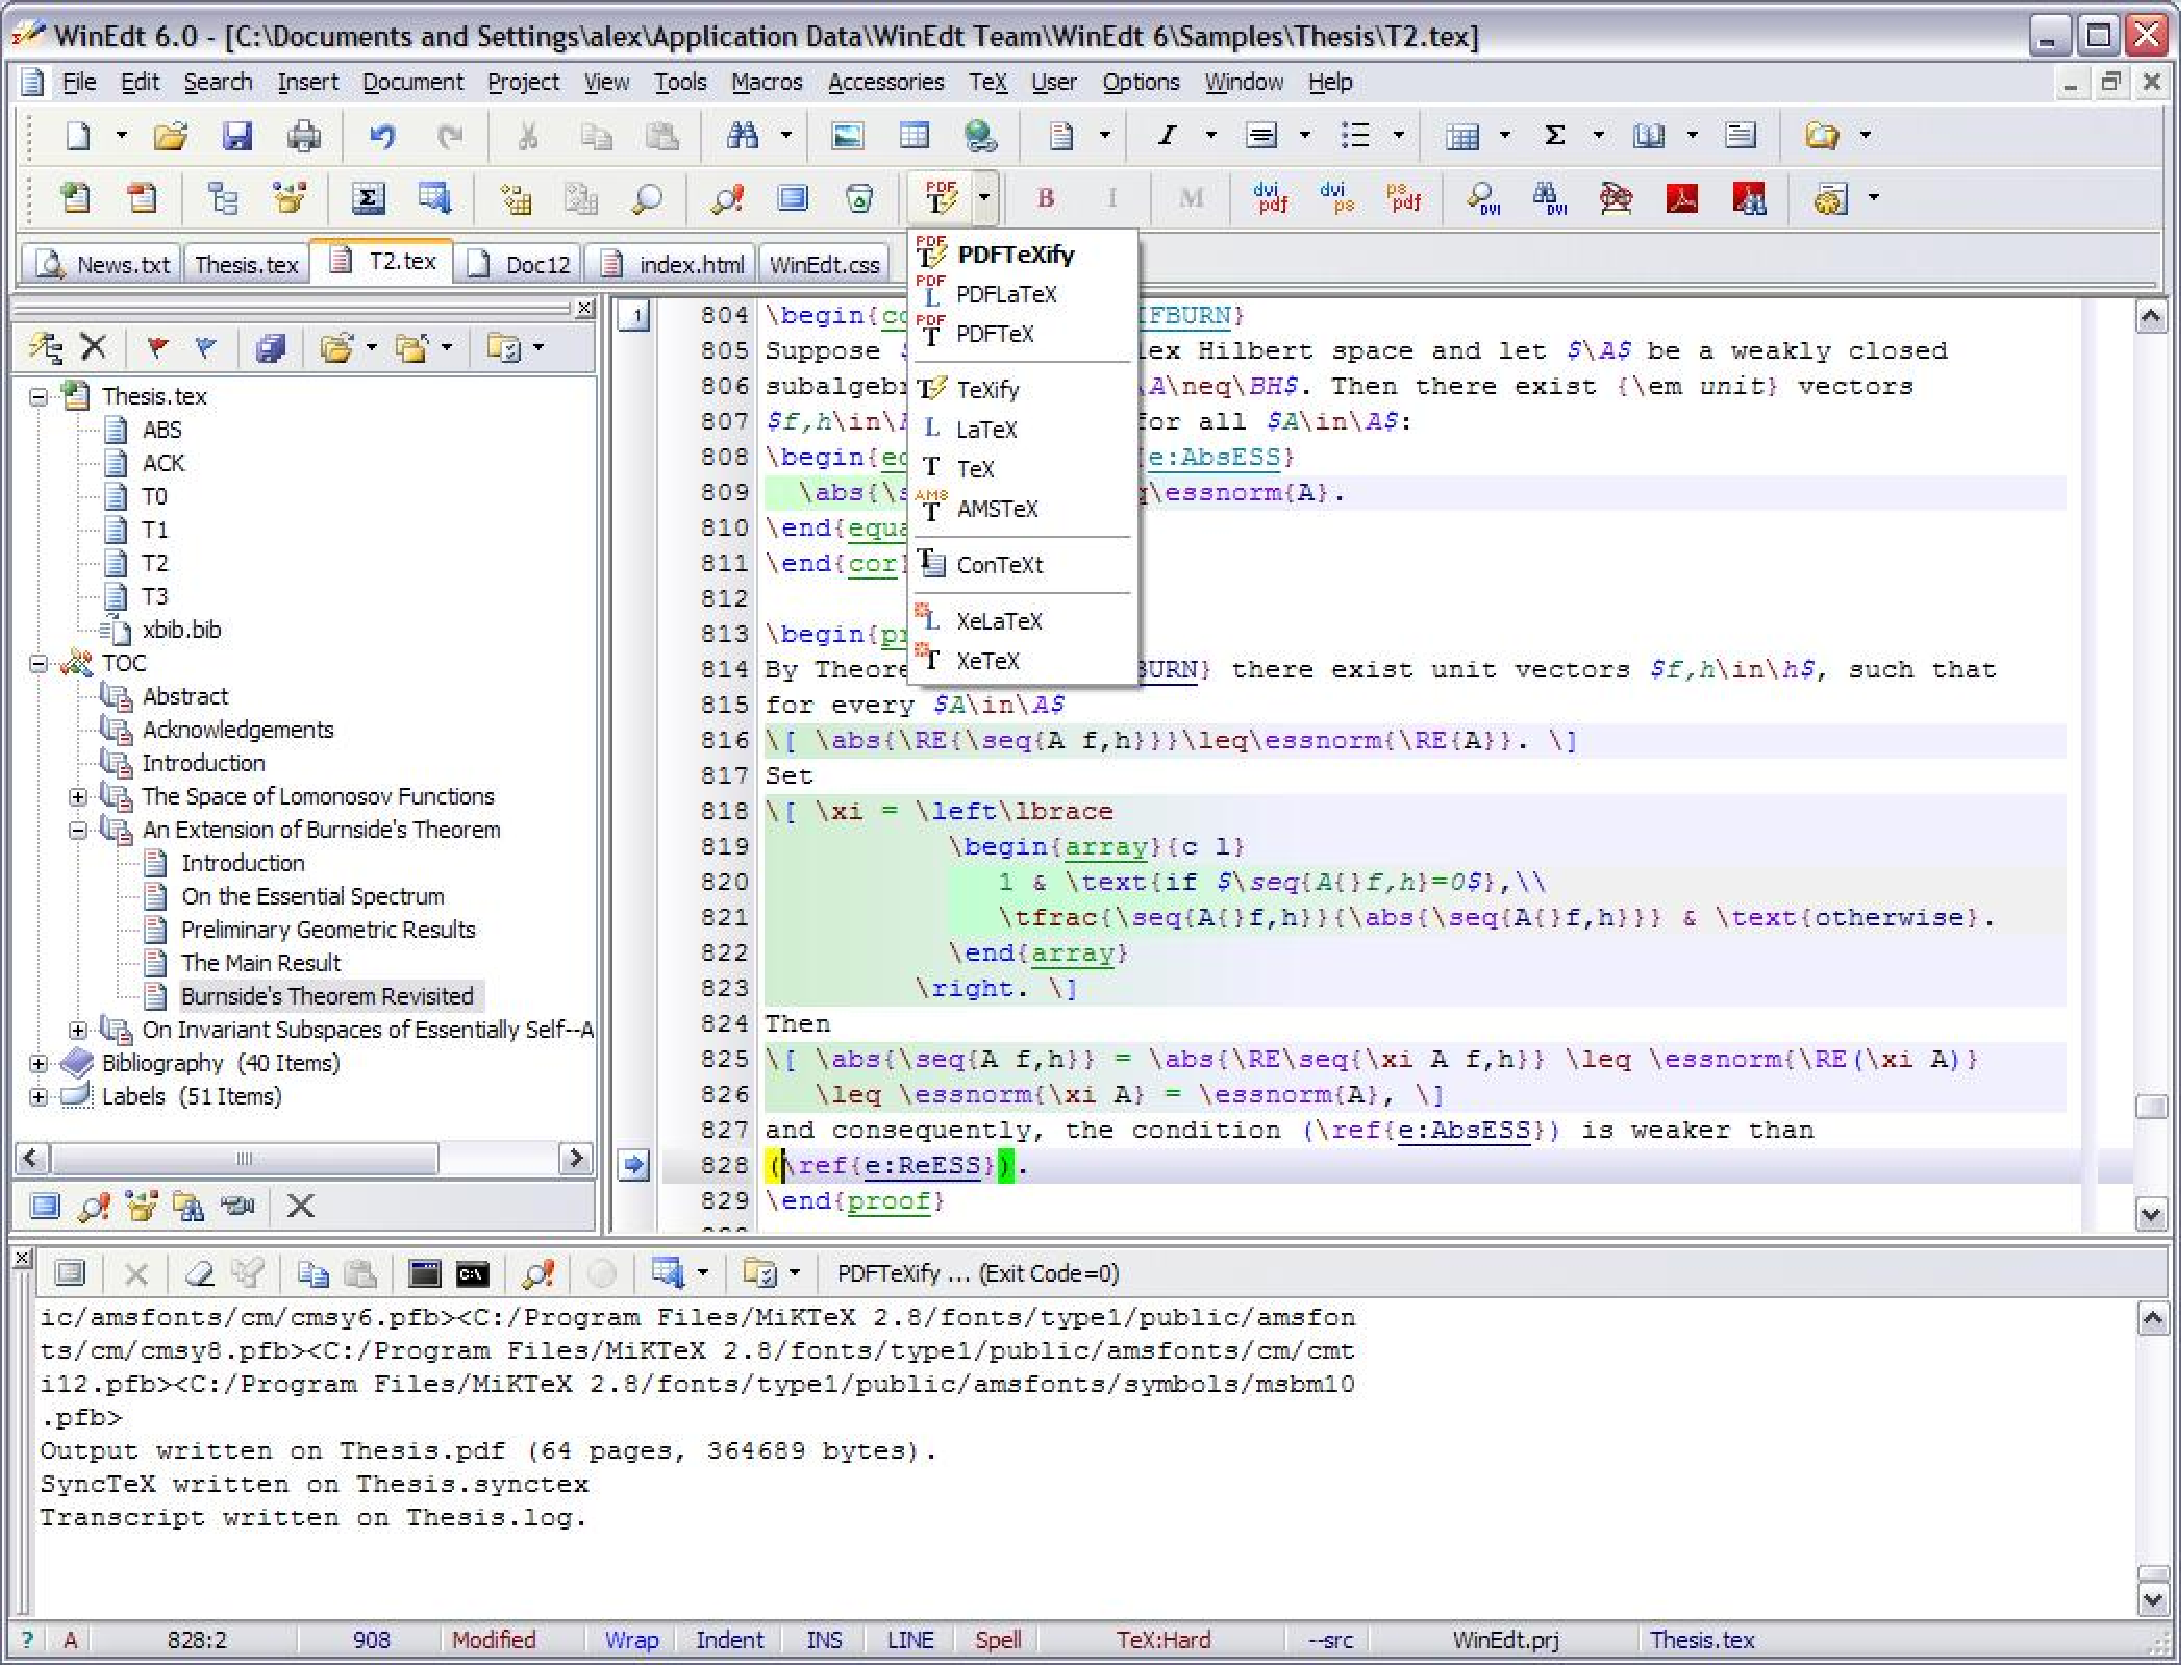
\includegraphics[width=0.65\textwidth]{img/WinEdt.pdf}
\end{itemize}
\end{frame}

\begin{frame}{\TeX{}nicCenter}
\begin{itemize}
\item Disponível somente para Windows
\item Veja: \url{http://www.texniccenter.org/}

\vspace{0.5cm}

\centering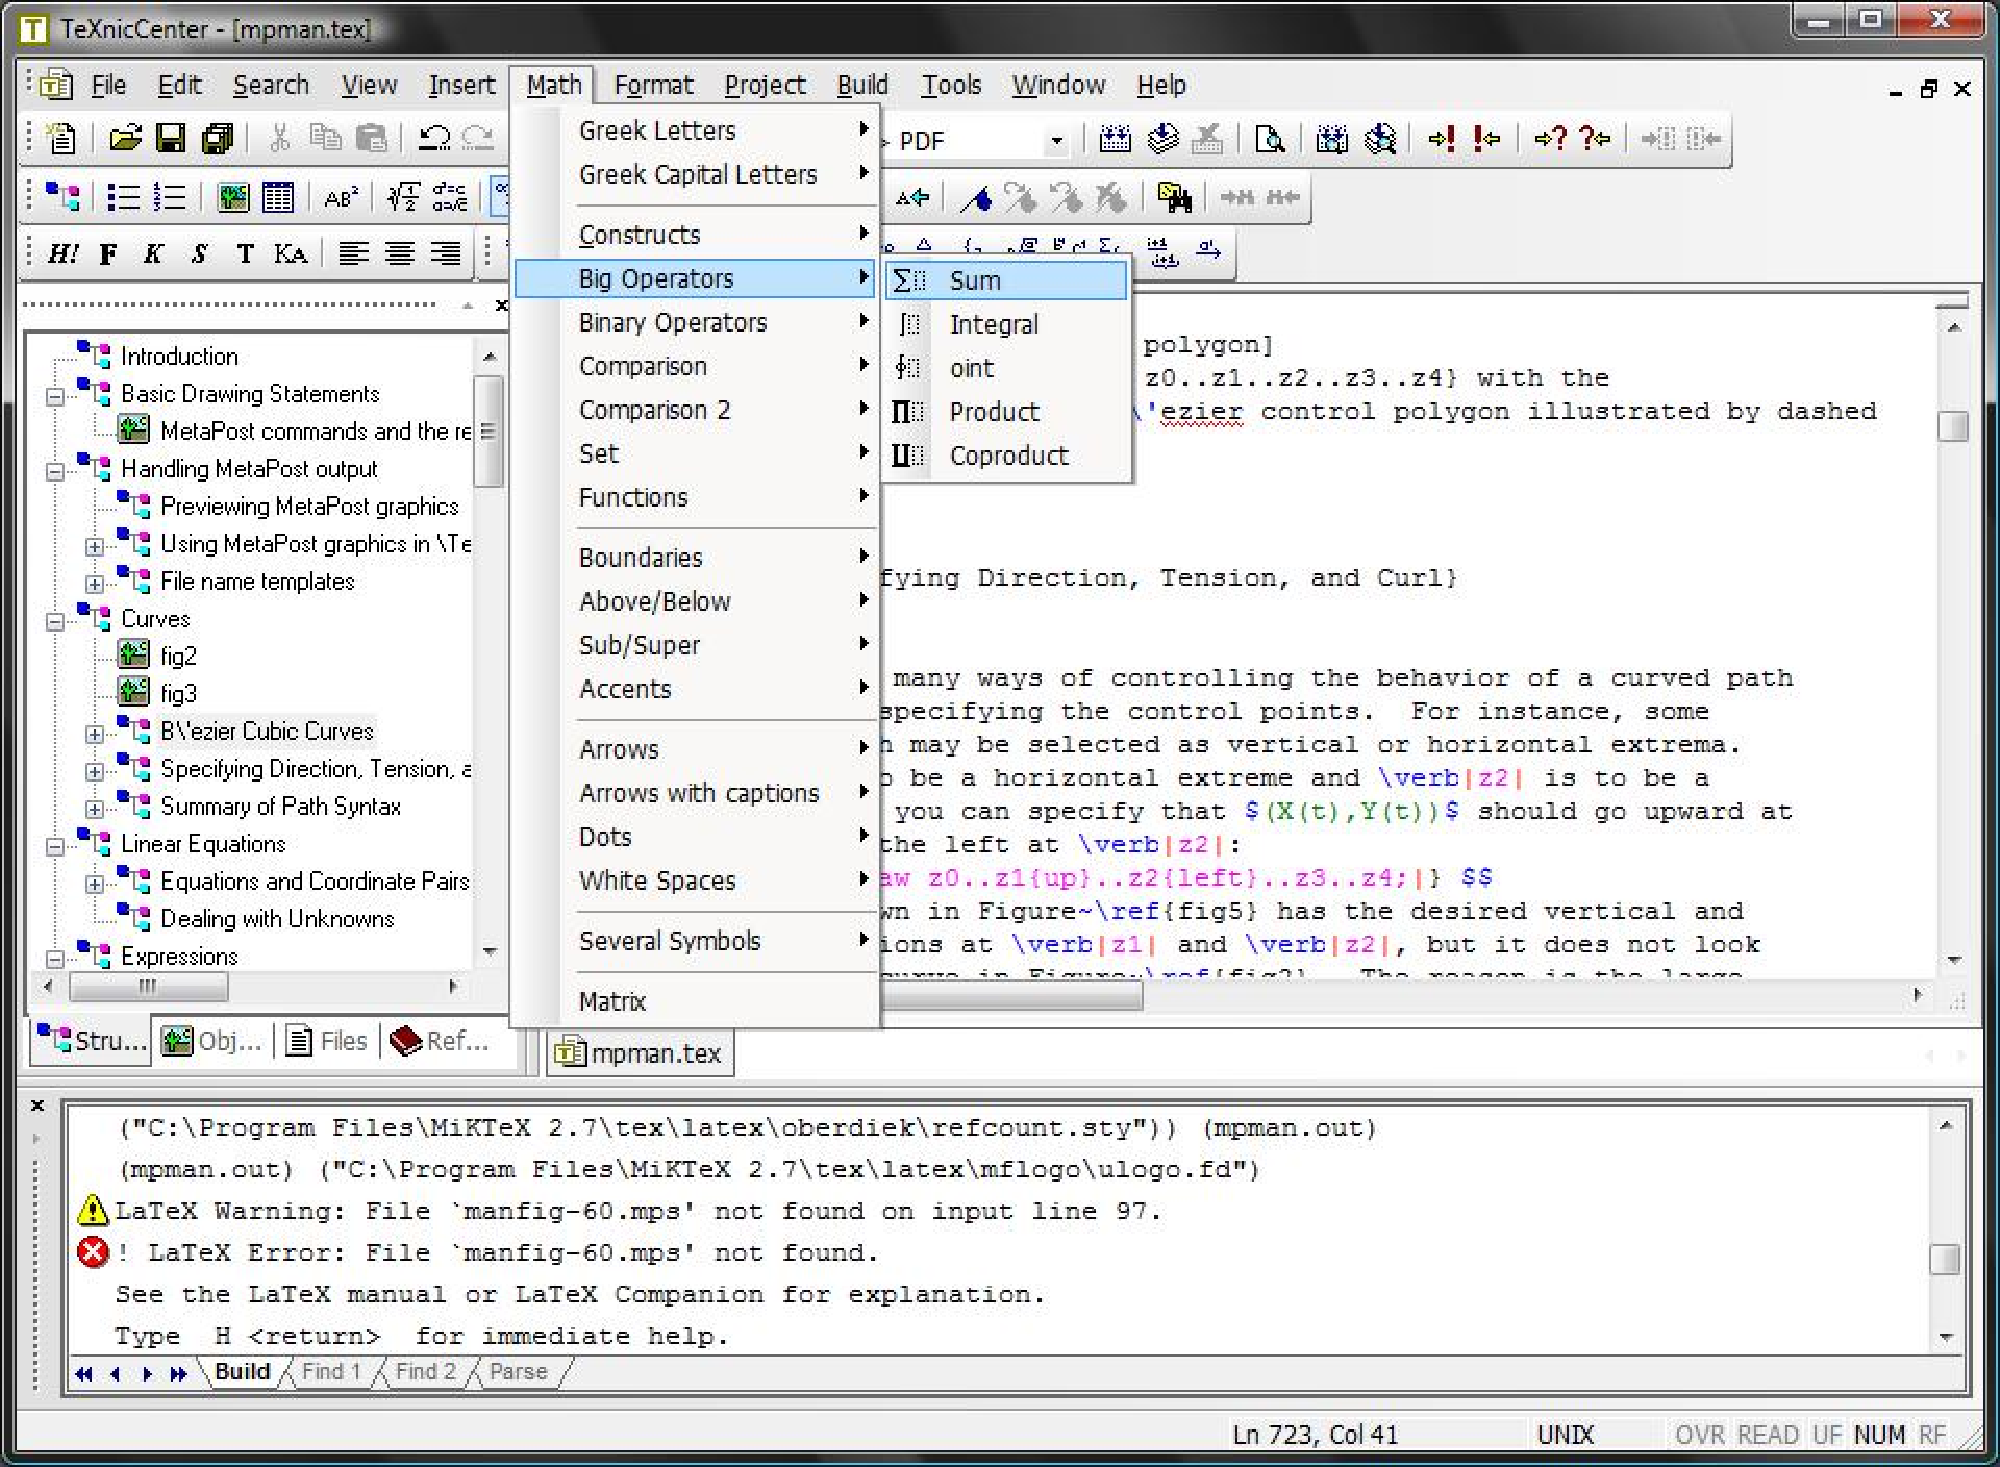
\includegraphics[width=0.70\textwidth]{img/texniccenter.pdf}
\end{itemize}
\end{frame}

\begin{frame}{ShareLaTex}
Editor On-Line: \url{http://sharelatex.com}
\begin{center}
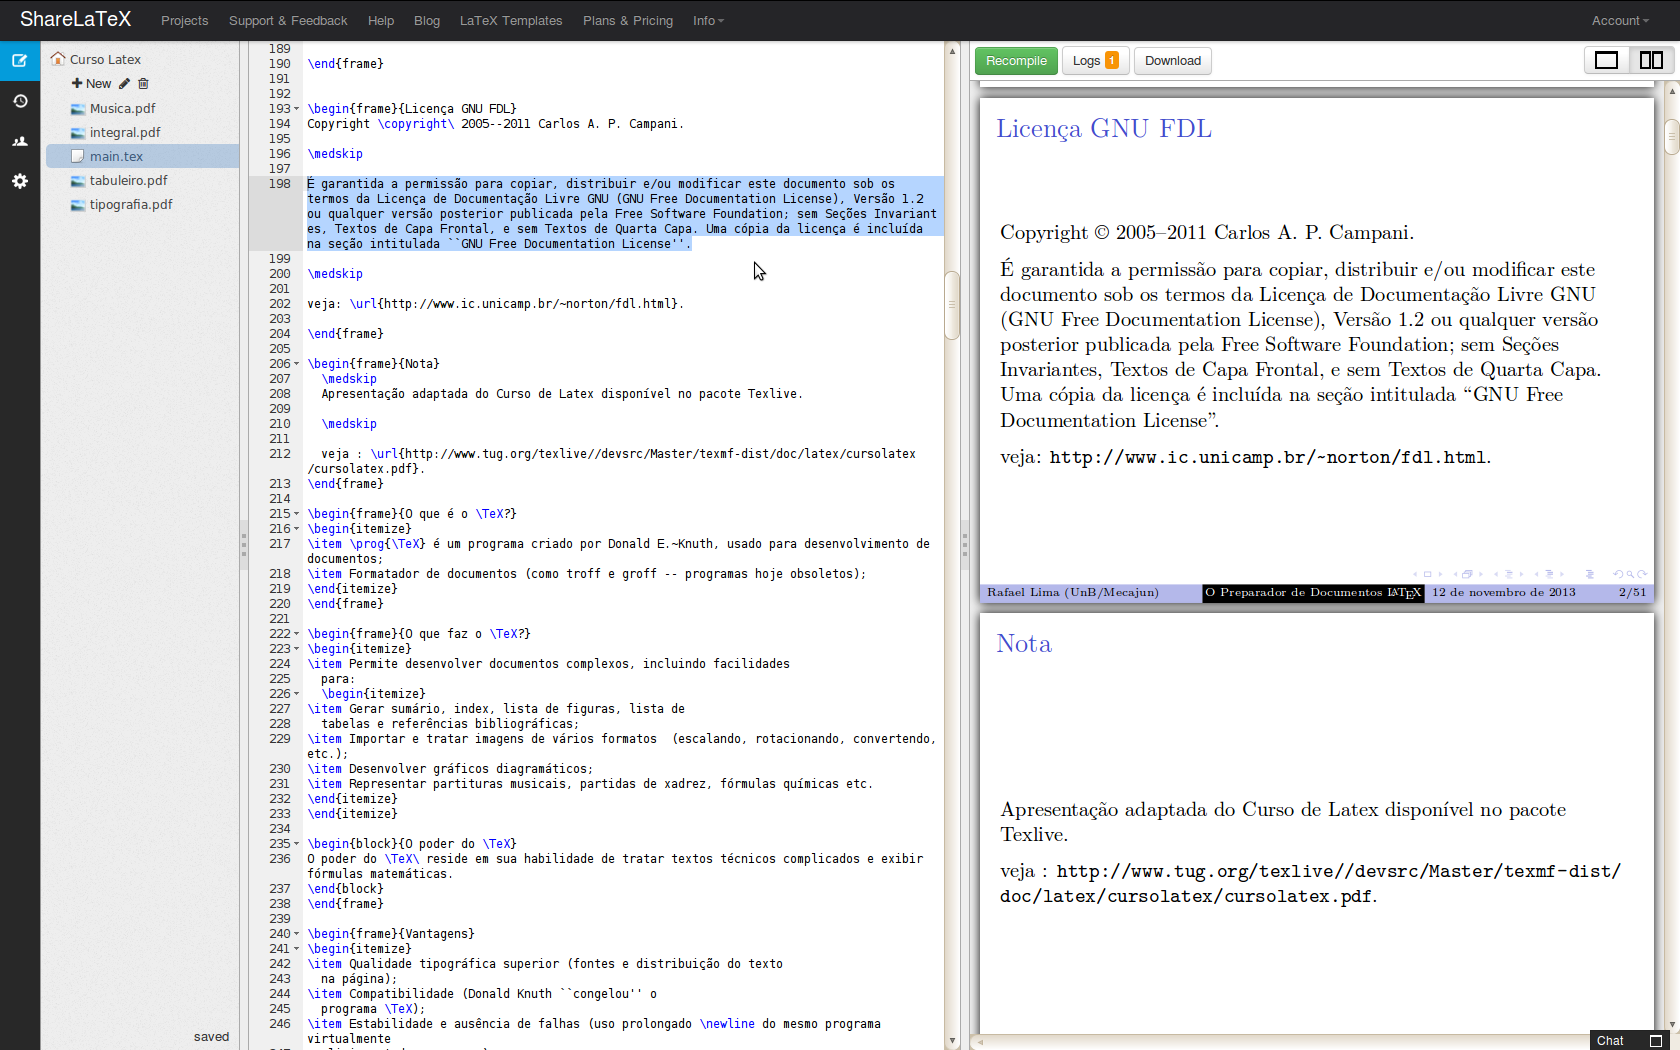
\includegraphics[width=0.85\textwidth]{img/sharelatex.png}
\end{center}
\end{frame}

\begin{frame}{LyX}
Editor WYSWG\footnote{WYSWG - What You See What You Get} para LaTeX % /TODO Explicar o termo WYSWG
\begin{center}
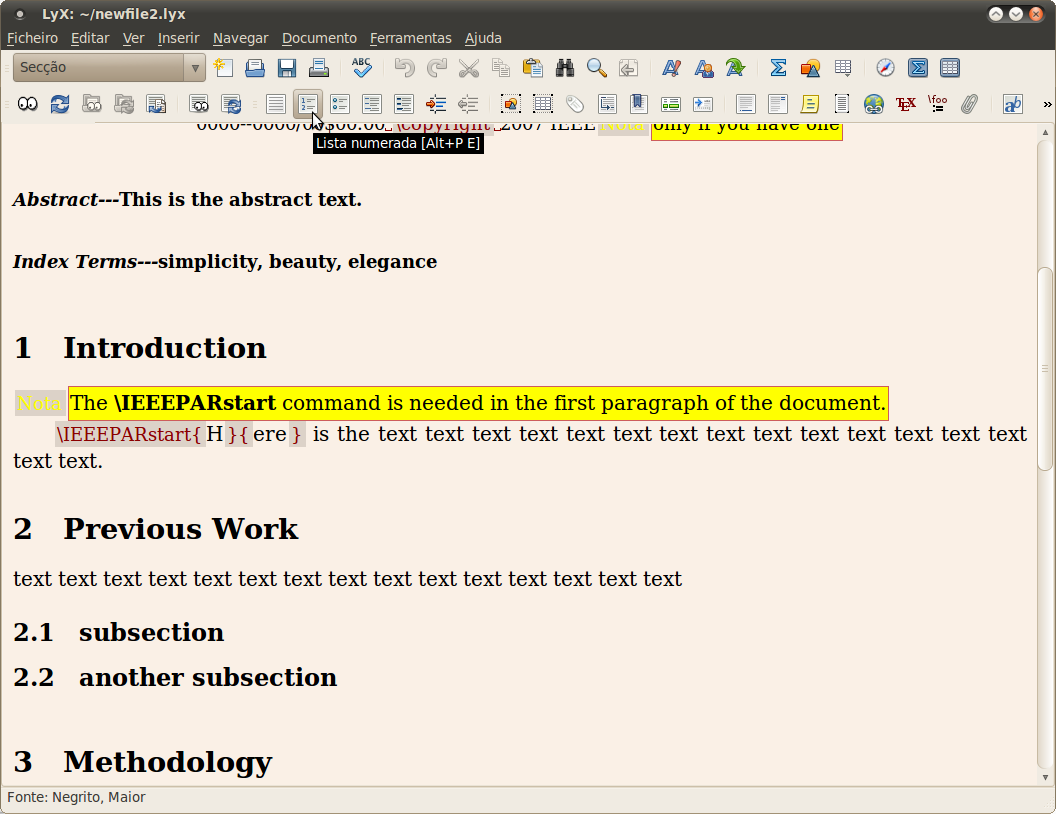
\includegraphics[width=0.70\textwidth]{img/LyX.png}
\end{center}
\end{frame}

\begin{frame}[fragile] % /TODO Verificar este slide
\frametitle{Compilando, visualizando e imprimindo}
\begin{itemize}
\item Compilação: Abrir o Terminal do Linux e usar o comando \verb+$ pdflatex teste.tex+ (para compilar, por exemplo, o arquivo \verb+teste.tex+) ou usar o menu \emph{TeX/TeX File} no \prog{Emacs}. No \prog{\TeX{works}} clicar no botão verde;
\item Visualização: \verb+$ xdg-open teste.pdf+ (o arquivo é recarregado automaticamente a cada modificação). Em alguns programas o resultado em .PDF aparece direitamente numa segunda janela;
\item Convertendo para html: \verb+$ latex2html teste.tex+;
\item Imprimindo: \verb+$ dvips teste.dvi+ ou \verb+$ lpr teste.ps+ no Terminal do Linux. Para imprimir no \prog{\TeX{Shop}} use \emph{File/Print}
\end{itemize}
\end{frame}

\begin{frame}{Estrutura e comandos \LaTeX}
\begin{LaTeXcode}[Estrutura geral]
\LCmdOptArg{documentclass}{opcionais}{classe}\n
declarações\n
\LCmdArg{begin}{document}\n
documento\n
\LCmdArg{end}{document}
\end{LaTeXcode}

\medskip

\begin{LaTeXcode}[Para trabalhar com arquivos grandes]
\LCmdArg{include}{nomearquivo}
\% inclui comandos de um arquivo\n \% gera nova página antes\nn
\LCmdArg{input}{nomearquivo} 
\% inclui comandos de um arquivo\n \% não gera nova página
\end{LaTeXcode}
\end{frame}

\begin{frame}{Estrutura dos comandos}
\begin{itemize}
\item Comandos \LaTeX{} são normalmente precedidos por \texttt{\textbackslash} e seguidos de parâmetros opcionais (delimitados por ``\texttt{[}`` e ``\texttt{]}'') e/ou parâmetros obrigatórios (delimitados por ``\texttt{\lb}'' e ``\texttt{\rb}'');
\begin{LaTeXcode}[Exemplos]
\LCmd{TeX}\n
\LCmd{LaTeX}\n
\LCmdArg{documentclass}{book}\n
\LCmdOptArg{documentclass}{12pt}{article}\n
\LCmdArg{begin}{document}
\end{LaTeXcode}

\bigskip

\item Uma excessão a esta regra é ``\texttt{\$}'' que delimita o ambiente matemático. Exemplo: \texttt{\$3+2\LCmdArg{sqrt}{2}\$}, que produz $3+2\sqrt{2}$.
\end{itemize}
\end{frame}

\begin{frame}{Espaços}
\begin{itemize}
\item Diversos espaços em branco, tabulações e novas linhas são desprezados (são considerados como um ``espaço branco simples'');
\item Os espaços adicionais são consumidos.
\end{itemize}
\end{frame}

\begin{frame}{Espaços após um comando \TeX}
Espaços após um comando serão consumidos até encontrar um caracter diferente de branco, resultando que
\begin{LaTeXcode}
\LCmd{TeX} é legal!
\end{LaTeXcode}
Produz:

\begin{LaTeXoutput}
\TeX é legal!
\end{LaTeXoutput}

Para evitar isto, use \texttt{\textbackslash\textvisiblespace}\footnote{O símbolo \texttt{\textvisiblespace}  serve para representar o espaço no texto fonte.} ou \texttt{\{\}}, que interrompe o consumo de espaços em branco, ou \texttt{\textasciitilde} (espaço em branco indivisível):
\begin{LaTeXcode}
\LCmd{TeX}\textbackslash\textvisiblespace é legal!\n
ou\n
\LCmd{TeX}\{\}\textvisiblespace é legal!\n
ou\n
\LCmd{TeX}\textasciitilde é legal!
\end{LaTeXcode}
\end{frame}

\begin{frame}{Delimitação de parágrafos}
Uma ou mais linhas em branco delimita os parágrafos:

\begin{LaTeXcode}[Exemplo]
Este é o\textvisiblespace\textvisiblespace\textvisiblespace\textvisiblespace primeiro \n parágrafo.\n

E este é o segundo!
\end{LaTeXcode}

Produz:
\begin{LaTeXoutput}
Este é o         primeiro
parágrafo.

E este é o segundo!
\end{LaTeXoutput}
\end{frame}

\begin{frame}{Comentários no arquivo fonte}
Comentários em \TeX\ são obtidos usando-se \texttt{\%}

Exemplo:
\begin{LaTeXcode}[Arquivo fonte com comentários]
Este é um exemplo\n
\% comentários são considerados\n
\% espaços em branco\n
de uso de comentários. \% fim do exemplo
\end{LaTeXcode}

Produz:
\begin{LaTeXoutput}
Este é um exemplo
% comentários são considerados
% espaços em branco
de uso de comentários. % fim do exemplo
\end{LaTeXoutput}
\end{frame}

\begin{frame}{Classes disponíveis}
\begin{itemize}
\item Principais classes disponíveis:
\begin{description}
\item [\Lcls{article}] Artigos curtos;
\item [\Lcls{report}] Artigos mais longos, monografias, relatórios;
\item [\Lcls{book}] Livros;
\end{description}

\medskip

\item Principais opções: 

\medskip

\begin{itemize}
\item \Lopt{11pt} -- fonte de 11 pontos;
\item \Lopt{12pt} -- fonte de 12 pontos;
\item \Lopt{twoside} -- imprime em ambos os lados da página;
\item \Lopt{twocolumn} -- produz saída em duas colunas.
\end{itemize}

\medskip

\item Lembre-se: \LCmdOptArg{documentclass}{opções}{classe}
\end{itemize}
\end{frame}

\begin{frame}{Estilos de página}
\begin{LaTeXcode}
\LCmdArg{pagestyle}{estilo}\n
ou\n
\LCmdArg{thispagestyle}{estilo}
\end{LaTeXcode}

Estilos disponíveis:

\begin{description}
\item [plain] número de página centralizado no rodapé;
\item [headings] capítulo corrente e número de página no cabeçalho;
\item [empty] cabeçalho e rodapé vazios;
\end{description}
\end{frame}

\begin{frame}{Ambientes}
O \LaTeX{} trabalha com \emph{ambientes}; o escopo de um ambiente é
definido pelos comandos \LCmdArg{begin}{\dots} e
\LCmdArg{end}{\dots}. Exemplos:

\begin{LaTeXcode}
\LCmdArg{begin}{document}
...
\LCmdArg{end}{document}
\end{LaTeXcode}
e
\begin{LaTeXcode}
\LCmdArg{begin}{center}
...
\LCmdArg{end}{center}
\end{LaTeXcode}
\end{frame}

\begin{frame}{Exemplo de um arquivo .TEX simples}
\begin{LaTeXcode}[Exemplo de arquivo .TEX]
\LCmdOptArg{documentclass}{12pt}{article}\n
\LCmdArg{begin}{document}\n
Oi, mundo!\n

Eu sou \LCmd{LaTeX}!\n
\LCmdArg{end}{document}
\end{LaTeXcode}
que produz na saída:

\begin{LaTeXoutput}
Oi, mundo!

Eu sou \LaTeX!
\end{LaTeXoutput}
\end{frame}

\begin{frame}{Usando pacotes}

\begin{itemize}
\item Amplia as funcionalidades do \LaTeX;
\item Modularidade;
\item \LOA{usepackage}[opções]{pacote};
\end{itemize}
\end{frame}

\begin{frame}{Usando pacotes}
\begin{LaTeXcode}[Exemplo]
\LCmdArg{documentclass}{article}\n
\LOA usepackage[brazilian]{babel}\n
\LOA usepackage[latin1]{inputenc}\n
\LOA usepackage[T1]{fontenc}\n
\LCmdArg{usepackage}{lmodern}\n
\LCmdArg{usepackage}{graphicx}\n
\LCmdArg{usepackage}{amsmath,amssymb}\n
\LCmdArg{usepackage}{indentfirst}\n
\LCmdArg{usepackage}{url}\n
\LCmdArg{begin}{document}\n
\dots\n
\LCmdArg{end}{document}
\end{LaTeXcode}
\end{frame}

\begin{frame}{Usando pacotes}\fontsize{10}{11}\selectfont
\begin{lista}
\item [babel] determina a língua usada no texto (\Lopt{brazilian}  é o português com as variantes brasileiras);
\item [inputenc] determina a codificação usada (use  \Lopt{latin1} no Linux, \Lopt{ansinew} no Windows e \Lopt{utf8} para a codificação universal UNICODE);
\item[fontenc] determina a codificação dos fontes usados na saída; para o português é importante usar a codificação \Lopt{T1};
\item[lmodern] escolhe um fonte vetorial com a codificação \Lopt{T1} (melhora a qualidade dos fontes no PDF);
\item [graphicx] permite incorporar imagens no texto (formatos PDF, JPG, PNG, MPS e EPS);
\item [amsmath e amssymb] fontes e símbolos  matemáticos adicionais da AMS;
\item [indentfirst] indentação em início do primeiro parágrafo de seção;
\item [url] permite colocar urls no texto usando o comando \LCmdArg{url}{http://\dots}.
\end{lista}

\end{frame}

\begin{frame}{Definindo divisões do texto}
\LaTeX\ gera automaticamente a numeração das seções, existindo os 
seguintes comandos para a sua numeração:

\begin{LaTeXcode}[Comandos de divisão do texto]
\LCmd{part}\n
\LCmd{chapter}\n
\LCmd{section}\n
\LCmd{subsection}\n
\LCmd{subsubsection}\n
\LCmd{paragraph}\n
\LCmd{subparagraph}
\end{LaTeXcode}

A classe \Lcls{article} não permite o comando \LCmd{chapter}.
\end{frame}

\begin{frame}{Divisões do texto}
\begin{LaTeXcode}[Exemplo]
\LCmdArg{documentclass}{article}\n
\LOA usepackage[brazilian]{babel} \LOA usepackage[utf8]{inputenc}\n
\LOA usepackage[T1]{fontenc} \LCmdArg{usepackage}{lmodern}\n
\LCmdArg{begin}{document}\n
\LCmdArg{section}{Introdução}\n
bla, bla, bla\n
\LCmdArg{section}{Usando o \LCmd{LaTeX}}\n
\LCmdArg{subsection}{Uso Básico}\n
bla, bla, bla\n
\LCmdArg{subsection}{Uso Avançado}\n
\LCmdArg{section}{Conclusão}\n
bla, bla, bla\n
\LCmdArg{end}{document}
\end{LaTeXcode}
\end{frame}

\begin{frame}{Símbolos especiais}
Os seguintes sete símbolos especiais podem ser facilmente obtidos 
pelos seguintes comandos:

\begin{center}
\begin{tabular}{r*6c}
\$ &\& &\% &\# &\_ &\{ &\} \\
\LCmd{\$} &\LCmd{\&} &\LCmd{\%} &\LCmd{\#} &\LCmd{\textunderscore} &\LCmd{\lb} &\LCmd{\rb}
\end{tabular}
\end{center}

Esses símbolos são especiais porque são usados em comandos na sintaxe de \LaTeX{} e não podem ser obtidos direitamente.
\end{frame}

\begin{frame}[fragile]
\frametitle{Acentos e cedilha no texto}
\begin{center}\let\tt\ttfamily
\begin{tabular}{*7c}
ò & ó & ô & ö & õ & ç & Ç \\
\LCmdArg{`}{o} &\LCmdArg{'}{o} &\LCmdArg{\textasciicircum}{o} &\LCmdArg{\string"}{o} &\LCmdArg{\textasciitilde}{o} &\LCmdArg{c}{c} &\LCmdArg{c}{C}
\end{tabular}
\end{center}
\end{frame}

\begin{frame}{Conversão automática dos acentos}
O pacote \texttt{inputenc} faz internamente a conversão automática dos acentos e o usuário não tem de preocupar-se com os comandos de acentuação:

\begin{center}
á $\longrightarrow$ \texttt{\LCmd{'}a}
\end{center}

No entanto, se não existirem recursos no teclado de sua máquina para acentuar, você ainda poderá acentuar seu texto usando os comandos.
\end{frame}

\begin{frame}{Especificação das línguas usadas no documento}
\begin{itemize}
\item O pacote babel especifica as línguas usadas no documento (\Lopt{brazilian}, \Lopt{english}, etc.), definindo, entre outras coisas, as regras de hifenação (separação silábica);
\item A última língua especificada entre as opções é a língua geral do documento;
\item Exemplo:
\begin{LaTeXcode}[Especificação das línguas do documento]
\LOA usepackage[italian,english,brazilian]{babel}
\end{LaTeXcode}
e a língua geral do documento é o português do Brasil.
\end{itemize}
\end{frame}

\begin{frame}{Seleção das línguas do documento}
\begin{itemize}
\item O documento pode ser composto somente nas línguas especificadas no pacote \Lsty{babel}; 
\item A distribuição \TeX\ Live possui suporte para quase 50 línguas;
\item Isso implica que o \LaTeX\ muda as palavras como ``Capítulo'', por exemplo, em ``Chapter'', dependendo da língua escolhida.
\item Pode-se compor um trecho de texto em inglês, em um documento em português, com:
\begin{LaTeXcode}[Seleção local da língua]
\LCmdArg{begin}{otherlanguage}\Larg{english}\n
English text\n
\LCmdArg{end}{otherlanguage}
\end{LaTeXcode}
\end{itemize}
\end{frame}

\begin{frame}{Seleção das línguas do documento}
Um pequeno pedaço de texto em inglês, envolto por texto em português,  pode-se compor com:
\begin{LaTeXcode}[Texto estrangeiro em linha]
texto em português \LCmdArg{foreignlanguage}{english}\Larg{English text}
outro texto em português \dots
\end{LaTeXcode}
\end{frame}

\begin{frame}{Hifenação (divisão silábica)}
A hifenação é feita automaticamente por \LaTeX, desde que o pacote babel tenha sido carregado. No caso de ocorrer uma hifenação incorreta, a correção é feita usando-se:
\begin{LaTeXcode}[Hifenação irregular]
\LCmdArg{hyphenation}{PYTHON com-pu-ta-dor} \% (usado na área\n \% de declarações/correção global)\nn
com\LCmd{-}pu\LCmd{-}ta\LCmd{-}ção \% (usado no corpo do texto/local)
\end{LaTeXcode}
\end{frame}

\begin{frame}{Produzindo texto}
\begin{itemize}
\item Aspas: Não use \texttt{\string"\dots\string"}; use \texttt{`{}`\dots'{}'} que produz ``\dots''. 
\item Apóstrofes: \texttt{d'alembertiano} produz d'alembertiano;
\item Hífens:
\begin{center}\let\tt\ttfamily
\begin{tabular}{ll}
\tt madeira-branca & madeira-branca \\
\tt linhas 117-{}-138 & linhas 117--138 \\
\tt verdadeiro-{}-{}-ou falso? & verdadeiro---ou falso? \\
\tt \$-3.2\$ & $-3.2$
\end{tabular}
\end{center}
\end{itemize}
\end{frame}

\begin{frame}{Reticências}
\begin{itemize}
\item Para exprimir uma reticência no texto, usa-se \LCmd{dots};
\item Note a diferença entre \texttt{...} que produz ... e \texttt{\string\dots} que produz \dots;
\item Três pontinhos não são adequados pois são interpretados como três sentenças vazias;
\item Na matemática existem várias reticências; na linha da base, no meio da linha, e vertical e diagonal nas matrizes:
\begin{center}
\begin{tabular}{ll}
\ldots 		& \LCmd{ldots} \\
\vdots 		& \LCmd{vdots} \\
$\ddots$ 	& \texttt{\$\string\ddots\$}\\
$a,\dots,z$	& \texttt{\$a, \string\ldots, z\$} ou \texttt{\$a, \string\dots, z\$} \\
$a+\dots+ z$	& \texttt{\$a+ \string\cdots+ z\$} ou \texttt{\$a+ \string\dots+ z\$} \\
\end{tabular}
\end{center}
\item \LCmd{dots} sempre produz a reticência adequada pelo contexto.
\end{itemize}
\end{frame}

\begin{frame}{Ligaduras}
\begin{itemize}
\item As ligaduras mas frequentes são:

\medskip

 ff fi fl ffi \ldots ao invés de f{}f f{}i f{}l f{}f{}i;
\item Para evitar use-se um grupo vazio: \texttt{f\{\}f} que produz f{}f.
\end{itemize}

 \bigskip

\begin{block}{Usando a lupa}
{\Huge ff fi fl ffi} \ldots ao invés de {\Huge f{}f f{}i f\mbox{}l f{}f{}i}.
\end{block}
\end{frame}

\begin{frame}{Mudando o estilo do texto}
\let\tt\ttfamily

\begin{tabular}{lll}
				& Comando		& Declaração \\
\textbf{Bold} & \tt\string\textbf\{\dots\}	& \tt\{\string\bfseries \dots\} \\
\texttt{Máquina de escrever} & \tt\string\texttt\{\dots\} & \tt\{\string\ttfamily \dots \}\\
\textit{Itálico} & \tt\string\textit\{\dots\}	& \tt\{\string\itshape\dots\} \\
\textsf{Sans serif} & \tt\string\textsf\{\dots\}& \tt\{\string\sffamily\dots\} \\
\textsc{Small Caps}	& \tt\string\textsc\{\dots\}& \tt\{\string\scshape\dots\} \\
Ênfase  & \tt\string\emph\{\dots\} & \tt\{\string\em \dots\}
\end{tabular}

\begin{itemize}
\item Deve-se observar que o ênfase não usa sublinhado\footnote{O sublinhado jamais é usado em tipografia.}, e é obtido com itálico se o texto é normal e normal se o texto é itálico;
\item Os comandos produzem seu efeito somente sobre seu argumento (escopo);
\item Comandos e/ou declarações podem ser acumulados: \\ \texttt{\string\textbf\{\string\itshape\ Itálico negro\}} produz \textbf{\itshape Itálico negro}.
\end{itemize}
\end{frame}

\begin{frame}{Serifas}
\begin{itemize}
\item As serifas são os pequenos traços ou hastes que ocorrem nos prolongamentos das letras;
\item Servem para guiar o olhar ao longo do texto;
\item As serifas na base das letras formam uma linha que serve como referência para o olho ``trafegar'' na linha de texto (como um trem no trilho);
\item Ela aumenta a legibilidade do corpo do texto\footnote{Jamais se usa fonte \emph{sans serif} no corpo do texto.}.

\begin{block}{Comparação}
\centering{\Large\string_\string_\textrm{Com serifa}\string_\string_ \hspace{2cm} \string_\string_\textsf{Sem serifa}\string_\string_}
\end{block}
\end{itemize}
\end{frame}

\begin{frame}{Mudando o tamanho dos fontes}
\let\tt\ttfamily

\begin{center}
\begin{tabular}{ll}
\tiny tiny & \tt\{\string\tiny\ \dots\} \\
\scriptsize scriptsize & \tt\{\string\scriptsize\ \dots\} \\
\footnotesize footnotesize & \tt\{\string\footnotesize\ \dots\} \\
\small small & \tt\{\string\small\ \dots\} \\
\normalsize normalsize &\tt\{\string\normalsize\ \dots\} \\
\large\strut large & \tt\{\string\large\ \dots\} \\
\Large\strut Large & \tt\{\string\Large\ \dots\} \\
\LARGE\strut LARGE & \tt\{\string\LARGE\ \dots\} \\
\huge\strut huge & \tt\{\string\huge\ \dots\} \\
\Huge\strut Huge & \tt\{\string\Huge\ \dots\}
\end{tabular}
\end{center}

\begin{block}{}
Escopo da definição delimitado pelo grupo.
\end{block}
\end{frame}

\begin{frame}{Alinhamento do texto}
Ambientes \emph{center}, \emph{flushleft} e \emph{flushright}:

\begin{center}
\Huge Centrado
\end{center}

\begin{flushleft}
\Huge Esquerda
\end{flushleft}

\begin{flushright}
\Huge Direita
\end{flushright}
\end{frame}

\begin{frame}{Sobre espaçamento}\fontsize{10}{12}\selectfont
\begin{itemize}
\item Para produzir espaço no texto pode-se usar ``\LCmd{\textvisiblespace}'', que representa o espaço simples;
\item Para produzir espaço negativo: \texttt{\string\!};
\item ``\texttt{\textasciitilde}'' produz um espaço que não pode ser dividido em uma quebra de linha; por exemplo: \texttt{fone:\ 51\textasciitilde5551234};
\item \TeX\ assume que sentenças terminam com ``.'', introduzindo um espaço adicional ao final da frase. O comando \LCmd{frenchspacing} desabilita este espaço adicional;
\item Para obter espaço vertical: \LCmdArg{vspace}{espaço} (não permite obter espaço no início de uma página) e \LCmdArg{vspace*}{espaço} (conserva o espaço no início de uma página);
\item \LCmdArg{hspace}{espaço} permite obter espaço horizontal dentro de uma linha;
\item Pode-se usar as dimensões em pontos (pt), polegadas (in), milímetros (mm), centímetros (cm) etc.
\end{itemize}
\end{frame}

\begin{frame}{Quebra de linha, parágrafo e página}


\begin{itemize}
\item Quebra de linha: \texttt{\string\\ } ou \texttt{\string\newline};
\item Quebra de página: \texttt{\string\newpage}.
\end{itemize}

\end{frame}

\begin{frame}{Notas de rodapé}


As notas de rodapé podem ser obtidas colocando-se, no lugar do 
texto onde deve ser referenciada a nota, o comando \LCmdArg{footnote}{Texto da nota}, tendo como argumento o texto da nota. 

\begin{LaTeXcode}[Exemplo]
42\LCmdArg{footnote}{A resposta para a vida o universo e tudo mais}
\end{LaTeXcode}

Produz a saída:
\begin{LaTeXoutput}
42\footnote{A resposta para a vida o universo e tudo mais}
\end{LaTeXoutput}
\end{frame}

\begin{frame}{Produzindo títulos de trabalhos}
\begin{LaTeXcode}[Declarações]
\LCmdArg{title}{Título}\n
\LCmdArg{author}{Autor}\n
\LCmdArg{date}{Data} ou \LCmdArg{date}{}
\end{LaTeXcode}

Observações:
\begin{itemize}
\item \texttt{\string\date\{\}} omite a data do documento;
\item Omitindo-se o comando \texttt{\string\date}, é tomada a data corrente da máquina.
\end{itemize}

\begin{LaTeXcode}[Produzindo]
\LCmd{maketitle}
\end{LaTeXcode}
\end{frame}

\begin{frame}{Exemplo de uso de título de trabalho}
\begin{LaTeXcode}[Estrutura no fonte]
\LCmdArg{documentclass}{book}\n
\LCmdArg{title}{O Guia do Mochileiro das Galáxias}\n
\LCmdArg{author}{Douglas Adams}\n
\LCmdArg{date}{}\n
\LCmdArg{begin}{document}\n
\LCmd{maketitle}\n

O Universo é tão grande que comparado a ele mesmo ele é infinitamente menor...
\LCmdArg{end}{document}
\end{LaTeXcode}
\end{frame}

\begin{frame}{Resultado da composição do título}
\begin{LaTeXoutput}[Estrutura produzida]
{\centering
{\Large O Guia do Mochileiro das Galáxias}\\[\baselineskip]
{Douglas Adams}\par}

\vspace{4\baselineskip}

O Universo é tão grande que comparado a ele mesmo ele é infinitamente menor...
\end{LaTeXoutput}
\end{frame}